\subsubsection{Test Run Trigger System}
\label{sec:testrun_trigger}
A block diagram of the HPS test run trigger is shown in Fig.~\ref{fig:trigger_diagram}.  
\begin{figure}[]
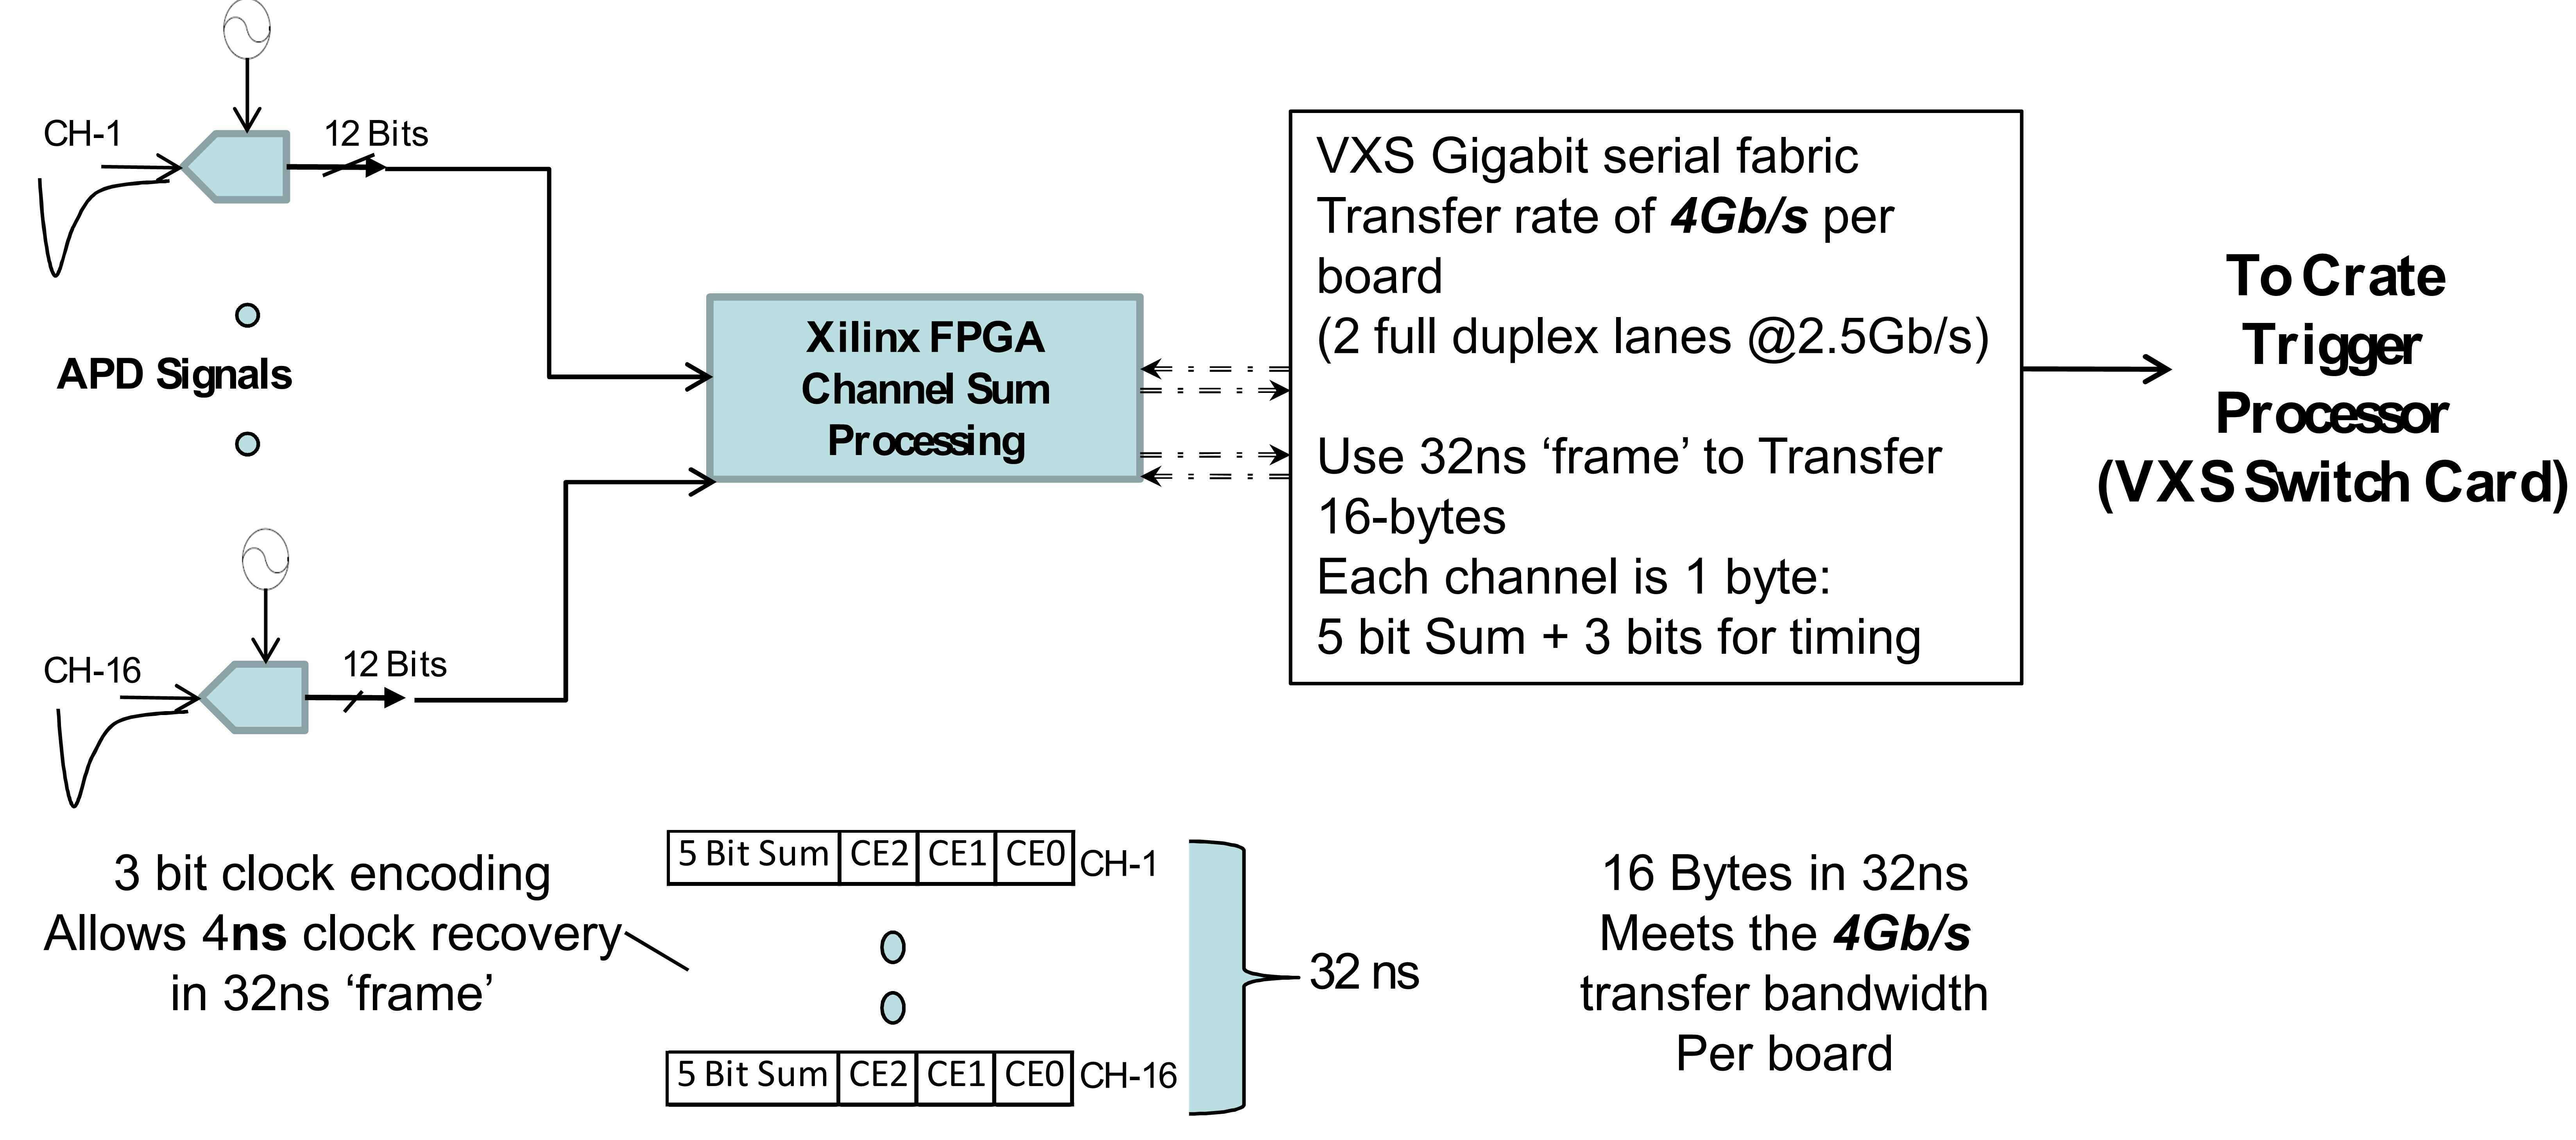
\includegraphics[scale=0.6]{test2012/trigger/HPSChanSum_001.jpg}
\caption{\small{Block diagram for the trigger system.}}
\label{fig:trigger_diagram}
\end{figure}
The trigger is based solely on information from the FADC boards and utilizes gigabit bandwidth to transport all the 
individual FADC channel sums (5-bits) and clock (3-bits) encoding bits. 
%The clock encoding bits report the 
%4~ns time period when the input signal crosses the programmable threshold within a 32~ns frame.  
The reported 5-bit channel sum value is extracted from the 17-bit register that contains the integrated (sum) 
signal value of the input channel. The channel integration occurs only if the input signal crosses the 
programmable threshold level: if the input signal does not cross threshold for a given 32~ns frame, the channel data is reported as zero.
The number of samples for a given channel integration cannot exceed the frame report latency time (128~ns or 32 samples) 
and only those samples above threshold are included. The processing and digitization of input signals are illustrated in Fig.~\ref{fig:trigsamples}. 
\begin{figure}[]
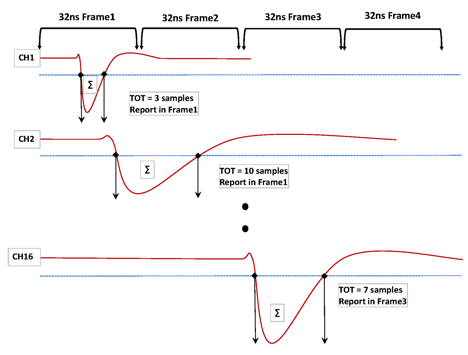
\includegraphics[scale=0.9]{test2012/trigger//trigger_pulse_samples}
\caption{\small{Example of input signals, and how they are integrated and digitized for the test run trigger.}}\label{fig:trigsamples}
\end{figure}
The time within a 32~ns frame where the input signal crosses threshold determines in which frame the 
integrated value is reported. Three clock encoding bits are used to time stamp the threshold crossing time to 
a 4~ns window.  
%In the example, the pulse for channel~2 crosses multiple frames.  The point where the signal crosses threshold determines the frame where the integration value will be reported for the given channel.  The number of points that are above threshold will be limited to 32. 
The trigger application only processes a single falling or rising edge per 32~ns frame. If multiple 
pulses arrive on a single channel within a 32~ns frame, they are not resolved and thus create a pile-up 
effect in the trigger system. However, multiple pulses per frame can be recovered from the readout data offline.

Information from each FADC channel are reported to the Crate Trigger Processor (CTP) through gigabit 
serial data streams. The sixteen serial data streams, one for each FADC board, were processed on a frame 
by frame basis. The cluster finding algorithm (see Sec.~\ref{sec:triggerdaq}) produces a serial data 
stream further processed by the Sub-System Processor (SSP), creating a readout trigger signal 
distributed to the FADC and SVT ATCA crates to initiate event readout. The system was designed to withstand 
a trigger accept rate higher than 50~kHz, above the limit set by the SVT DAQ.  

For the test run, the simplified trigger logic in the SSP was a simple threshold: the trigger was designed 
to fire on a single cluster with energy exceeding a given threshold. However, the full trigger described in 
Ref.~\cite{HPS_tPROP} was implemented and tested.
